\documentclass{article}
\usepackage[pdftex]{graphicx}
\usepackage{listings}
\usepackage{xcolor}
\lstset{basicstyle=\ttfamily,
  showstringspaces=false,
  commentstyle=\color{red},
  keywordstyle=\color{blue}
}
\begin{document}

\author{Jon Robison}
\title{CS595 Assignment 5}
\maketitle

Q1.  Determine if the friendship paradox holds for your Facebook account.\\
Create a graph of the number of friends (y-axis) and the friends sorted\\
by number of friends (x-axis).  (The friends don't need to be labeled \\
on the x-axis.)  Do include yourself in the graph and label yourself\\
accordingly.\\
\\
Compute the mean, standard deviation, and median of the number of friends\\
that your friends have. \\*

See Appendix A for translator\\
Average: 639.065843621 \\
Std deviation: 465.913488086 \\
Median: 535.0 \\
\graphicspath{{q1/}}
\begin{figure}
  \centering
  \caption{Friend count}
  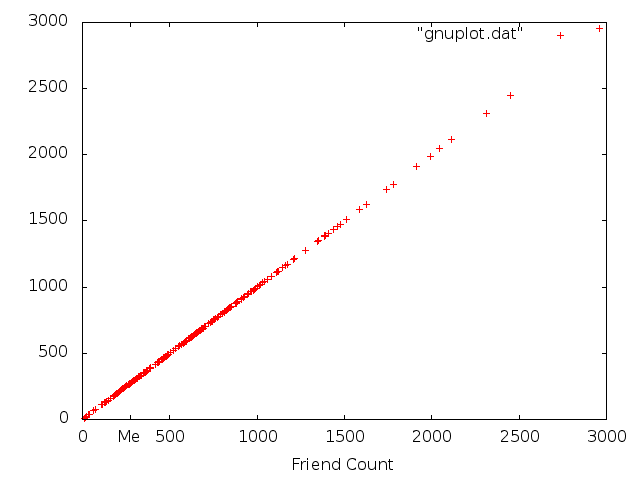
\includegraphics[scale=.3]{scatter.png}
\end{figure}
\clearpage

Q2. Determine if the friendship paradox holds for your Twitter account.\\
Since Twitter is a directed graph, use ``followers'' as value you measure\\
(i.e., ``do your followers have more followers than you?'').\\
\\
Generate the same graph as in question 1, and calcuate the same \\
mean, standard deviation, and median values.\\
\\*

Q3 EC. Repeat question 1, but with your LinkedIn profile\\
\\*

Q4 EC. Repeat question 2, but change ``followers'' to ``following''?  In\\
other words, are the people I am following following more people?\\
\\*

\newpage
\appendix
Appendix A
\lstinputlisting[language=python]{q1/createPlot.py}

\end{document} 
